\documentclass[12pt, a4paper, brazil]{article}

\usepackage{sbc-template}
\usepackage[utf8]{inputenc}
\usepackage[brazilian]{babel}
\usepackage[T1]{fontenc}
\usepackage{graphicx,url}
\usepackage{microtype}
\usepackage{float}
\usepackage{booktabs}
\usepackage{caption}
\usepackage{amsmath}

\sloppy

\title{Comparação entre as Estratégias Gulosa e de Tentativa e Erro (Backtracking) no Problema do Caminho em Labirinto}

\author{João Vitor Santana Lima e Samuel Torres Vieira da Silva}


\address{Departamento de Sistemas de Informação -- Universidade Federal do Piauí (UFPI) \\ 64.600-000 -- Picos -- PI -- Brasil
  \email{\{joao.vitor.1, samuel.vieira\}@ufpi.edu.br}
}

\begin{document}

\maketitle

\begin{resumo}
Este trabalho compara duas estratégias de projeto de algoritmos, a abordagem Gulosa e a de Tentativa e Erro (Backtracking), aplicadas ao problema do caminho em labirinto, no qual se busca ligar o canto superior esquerdo ao canto inferior direito de uma grade com paredes. A avaliação foi conduzida sobre dois casos de teste gerados com semente fixa (labirintos 6$\times$6 e 10$\times$10), medindo-se a qualidade da solução, o tempo de execução, o número de decisões e o consumo de memória. Os resultados mostram que a estratégia gulosa é ordens de grandeza mais rápida, porém não garante a solução ótima: no labirinto 6$\times$6 ela encontrou um caminho 20\% mais longo que o mínimo e, no 10$\times$10, ficou presa em um beco sem saída e não encontrou solução alguma. O backtracking, por explorar exaustivamente o espaço de busca e desfazer decisões, encontrou o caminho ótimo em ambos os casos, ao custo de tempo, número de decisões e memória substancialmente maiores.
\end{resumo}

\section{Introdução e Metodologia}
O problema do caminho em labirinto consiste em encontrar um trajeto que ligue a célula inicial (canto superior esquerdo) à célula objetivo (canto inferior direito) de uma grade quadrada, movendo-se apenas por células livres nas quatro direções ortogonais e desviando das paredes~\cite{cormen2009}. Neste trabalho, esse problema é resolvido por duas estratégias distintas, cujos desempenhos são comparados empiricamente.

A estratégia gulosa constrói uma única tentativa de caminho: a cada passo, dentre as células vizinhas livres ainda não visitadas, escolhe aquela cuja distância de Manhattan até o objetivo é a menor, avançando sempre na direção que parece localmente mais promissora~\cite{cormen2009}. A decisão nunca é revista, pois o algoritmo não retrocede. Caso chegue a uma célula sem vizinhos disponíveis antes de alcançar o objetivo, ele declara que não há solução.

A estratégia de tentativa e erro (backtracking) é uma técnica clássica de projeto de algoritmos baseada em busca exaustiva com retrocesso~\cite{aho1974design}. Ela realiza uma busca em profundidade que explora sistematicamente todos os caminhos possíveis, marcando as células visitadas e desfazendo cada decisão ao retornar da recursão~\cite{sedgewick2011, weiss2014datastructures}. Sempre que alcança o objetivo, registra o caminho e mantém o mais curto; uma poda descarta ramos que já não podem superar a melhor solução corrente. Ao percorrer todo o espaço de busca viável, o backtracking garante a obtenção do caminho ótimo (de menor número de passos).

Os labirintos foram gerados aleatoriamente com semente fixa (garantindo reprodutibilidade) e densidade de paredes de 28\%, descartando-se as grades sem caminho viável entre início e fim. A avaliação empírica complementa a análise teórica, evidenciando diferenças práticas de desempenho que a notação assintótica isoladamente não captura~\cite{mcconnell2008code}. Para cada caso foram medidos: o resultado obtido, se a solução é ótima, o tempo médio de execução (média de 21 repetições, via \texttt{perf\_counter}), o número de decisões tomadas e o pico de memória (via \texttt{tracemalloc}). As seções a seguir apresentam dois casos de teste representativos: um labirinto 6$\times$6 e um 10$\times$10.

\section{Casos de Teste e Resultados}

\subsection{Labirinto 6$\times$6}
A Figura~\ref{fig:lab6} ilustra o labirinto 6$\times$6. O caminho ótimo (em azul) tem 10 passos, enquanto o rastro do guloso (em laranja) percorre 12 passos: ele chega ao objetivo, mas por uma rota mais longa. A Tabela~\ref{tab:caso6} consolida as métricas.

\begin{figure}[H]
    \centering
    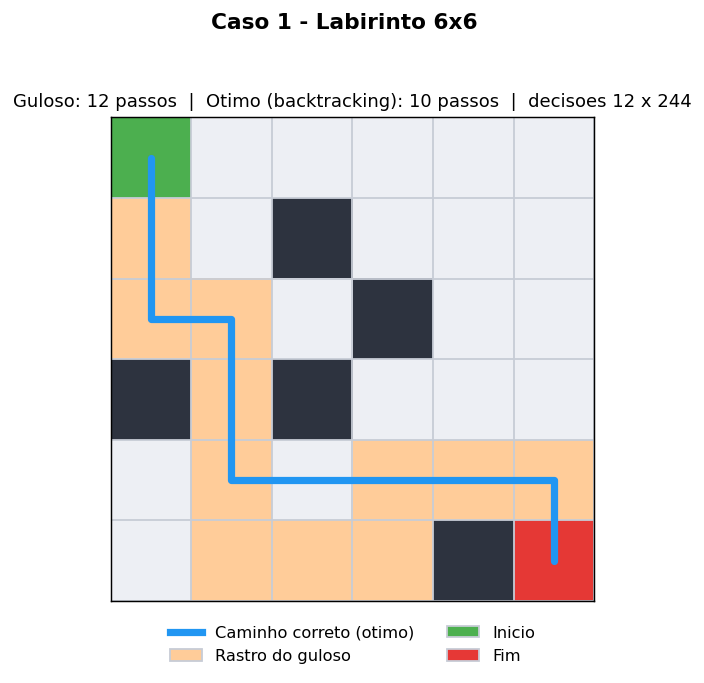
\includegraphics[width=0.62\linewidth]{figures/labirinto_6x6.png}
    \caption{Labirinto 6$\times$6: caminho ótimo (azul, 10 passos) e rastro do guloso (laranja, 12 passos).}
    \label{fig:lab6}
\end{figure}

\begin{table}[H]
\centering
\caption{Comparativo entre Guloso e Backtracking no Labirinto 6$\times$6}
\label{tab:caso6}
\begin{tabular}{lcc}
\toprule
\textbf{Critério} & \textbf{Guloso} & \textbf{Backtracking} \\
\midrule
Resultado obtido            & Caminho com 12 passos & Caminho com 10 passos \\
Melhor solução encontrada   & Não (2 passos a mais) & Sim (ótimo)           \\
Tempo de execução (ms)      & 0,0175                & 0,1867                \\
Número de decisões          & 12                    & 244                   \\
Memória de pico (bytes)     & 3.164                 & 10.280                \\
\bottomrule
\end{tabular}
\end{table}

Neste caso, o guloso é cerca de 10,7 vezes mais rápido e toma 20 vezes menos decisões, mas entrega um caminho 20\% mais longo que o ótimo. O backtracking encontra o caminho mínimo, porém explora 244 estados até garantir a otimalidade.

\subsection{Labirinto 10$\times$10}
A Figura~\ref{fig:lab10} mostra um caso em que o guloso falha completamente. Guiado pela distância de Manhattan, ele desce em linha reta pela coluna da esquerda e fica preso em um beco sem saída (marcado com um X vermelho), após apenas 9 decisões, declarando que não há solução. O backtracking, por sua vez, encontra o caminho ótimo de 18 passos. A Tabela~\ref{tab:caso10} resume os resultados.

\begin{figure}[H]
    \centering
    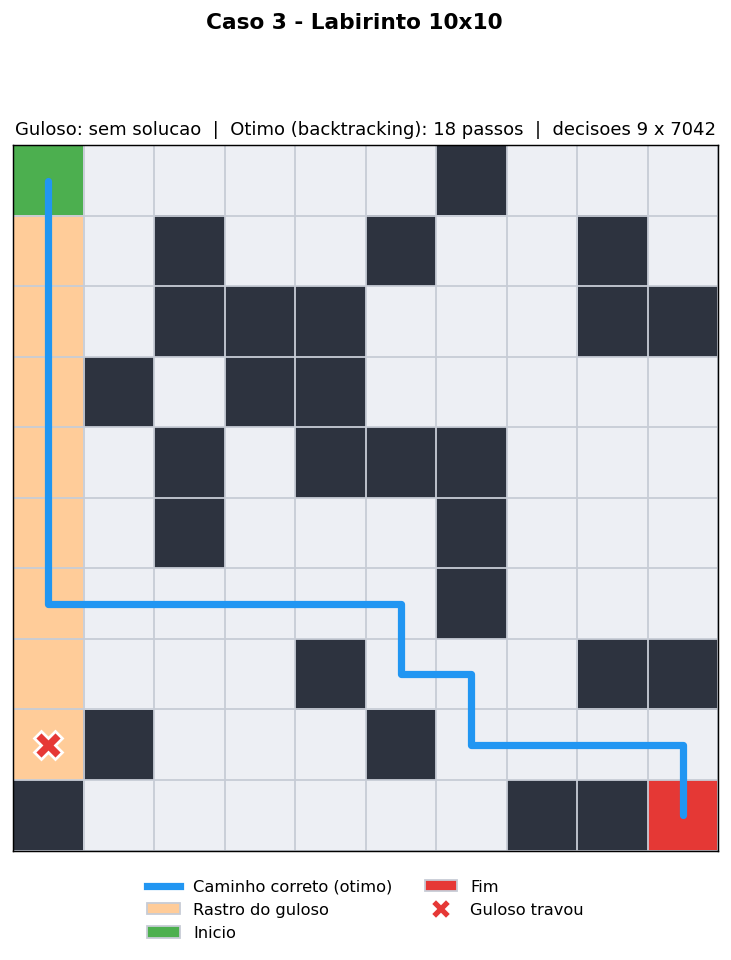
\includegraphics[width=0.58\linewidth]{figures/labirinto_10x10.png}
    \caption{Labirinto 10$\times$10: o guloso trava em um beco sem saída (X vermelho) e não encontra solução; o backtracking encontra o caminho ótimo (azul, 18 passos).}
    \label{fig:lab10}
\end{figure}

\begin{table}[H]
\centering
\caption{Comparativo entre Guloso e Backtracking no Labirinto 10$\times$10}
\label{tab:caso10}
\begin{tabular}{lcc}
\toprule
\textbf{Critério} & \textbf{Guloso} & \textbf{Backtracking} \\
\midrule
Resultado obtido            & Sem solução     & Caminho com 18 passos \\
Melhor solução encontrada   & Não encontrou   & Sim (ótimo)           \\
Tempo de execução (ms)      & 0,0121          & 5,6292                \\
Número de decisões          & 9               & 7.042                 \\
Memória de pico (bytes)     & 1.428           & 8.572                 \\
\bottomrule
\end{tabular}
\end{table}

Aqui a diferença de qualidade é máxima: o guloso não encontra caminho algum, embora exista uma solução de 18 passos. O preço da garantia do backtracking também cresce muito com o tamanho do labirinto, pois o número de caminhos a enumerar aumenta de forma combinatória~\cite{knuth1998}: foram 7.042 decisões (cerca de 780 vezes mais que o guloso) e um tempo aproximadamente 465 vezes maior.

\section{Respostas às Perguntas}

\subsection{O algoritmo guloso encontra sempre a melhor solução? A solução gulosa é ótima ou apenas boa?}
Não. Em nenhum dos casos de teste o guloso produziu a solução ótima. No labirinto 6$\times$6 ele encontrou um caminho, mas subótimo (12 passos contra 10 do ótimo, ou seja, 20\% mais longo); no 10$\times$10 ele sequer encontrou solução. Portanto, a solução gulosa é, no melhor cenário, apenas \textbf{boa} (uma aproximação rápida) e, no pior, \textbf{inexistente}, pois nunca há garantia de otimalidade.

\subsection{Em quais situações ele falha e por quê?}
Foram observados dois modos de falha:
\begin{itemize}
    \item \textbf{Subotimalidade (6$\times$6):} a escolha localmente melhor (menor distância de Manhattan) conduz a um caminho globalmente mais longo. Como a heurística ignora as paredes, o movimento míope de ``chegar mais perto agora'' força um desvio maior adiante.
    \item \textbf{Falha total / beco sem saída (10$\times$10):} como o guloso nunca retrocede, ao entrar em uma região sem vizinhos livres não visitados ele não tem como sair e declara ``sem solução'', mesmo existindo caminho.
\end{itemize}
A causa raiz é que o problema do caminho mínimo em labirinto \textbf{não possui a propriedade da escolha gulosa}: uma decisão localmente ótima não garante uma solução globalmente ótima (nem sequer viável), e o comprometimento irrevogável do guloso o impede de corrigir uma escolha inicial ruim~\cite{cormen2009}.

\subsection{O backtracking encontra a solução ótima?}
Sim. Em ambos os casos ele retornou o caminho de menor comprimento (10 e 18 passos), o que é garantido pela poda que sempre mantém a menor solução encontrada. Essa garantia decorre de explorar exaustivamente o espaço de busca viável e desfazer decisões, ao custo de um número de decisões, tempo e memória muito maiores, por exemplo, 7.042 decisões e 5,6292~ms no labirinto 10$\times$10, contra 9 decisões e 0,0121~ms do guloso.

\subsection{Quanto as soluções diferem?}
A Tabela~\ref{tab:diferencas} resume as diferenças por caso de teste. O guloso vence por larga margem em tempo, número de decisões e memória, mas perde em qualidade: ou entrega um caminho subótimo, ou falha por completo.

\begin{table}[H]
\centering
\caption{Diferenças entre as soluções por caso de teste}
\label{tab:diferencas}
\begin{tabular}{lcc}
\toprule
\textbf{Aspecto} & \textbf{Labirinto 6$\times$6} & \textbf{Labirinto 10$\times$10} \\
\midrule
Qualidade (passos)        & 12 vs 10 ($+$2 passos, $+$20\%)          & sem solução vs 18 passos \\
Decisões (BT / Guloso)    & 244 vs 12 ($\approx 20\times$)          & 7.042 vs 9 ($\approx 780\times$) \\
Tempo (BT / Guloso)       & $\approx 10{,}7\times$ mais lento       & $\approx 465\times$ mais lento \\
Memória (BT / Guloso)     & $\approx 3{,}2\times$ maior             & $\approx 6{,}0\times$ maior \\
\bottomrule
\end{tabular}
\end{table}

\subsection{Pergunta sorteada: mostre um caso onde o guloso falha}
O labirinto 10$\times$10 (Figura~\ref{fig:lab10}) é o exemplo mais claro: seduzido pela heurística da distância de Manhattan, o guloso desce em linha reta pela coluna da esquerda e fica preso em um beco sem saída após 9 movimentos, retornando ``sem solução'', enquanto o backtracking encontra um caminho de 18 passos. O labirinto 6$\times$6 (Figura~\ref{fig:lab6}) mostra uma falha mais branda: o guloso alcança o objetivo, mas por um caminho subótimo de 12 passos, contra os 10 do ótimo.

\section{Conclusão}
Os experimentos evidenciam o compromisso (\textit{trade-off}) entre as duas estratégias. A abordagem gulosa é extremamente rápida e econômica, pois toma uma única sequência de decisões locais, mas não oferece garantia de otimalidade nem de completude: no labirinto 6$\times$6 produziu um caminho 20\% mais longo que o ótimo e no 10$\times$10 falhou por ficar presa em um beco sem saída. A abordagem de tentativa e erro (backtracking) sempre encontrou o caminho ótimo, ao custo de um número de decisões, tempo e memória muito superiores, que ainda crescem rapidamente com o tamanho do labirinto. Conclui-se que a estratégia gulosa só é adequada quando uma solução aproximada e rápida é aceitável e o domínio garante a propriedade da escolha gulosa; quando a otimalidade ou a garantia de encontrar solução são necessárias, o backtracking (ou outros métodos de busca completos) torna-se indispensável~\cite{cormen2009, sedgewick2011}.


\bibliographystyle{sbc}
\bibliography{sbc-template}

\end{document}
